\documentclass[a4paper]{article}
\usepackage{exercise}
%um nur aufgaben zu zeigen
%\usepackage[noanswer]{exercise} 
\usepackage{../images/preamble}
\usepackage{rotating}
\usetikzlibrary{decorations.pathmorphing}
\usetikzlibrary{decorations.markings}
\usetikzlibrary{arrows}
\usetikzlibrary{shapes.geometric}
\newcommand{\midarrow}{\tikz \draw[-triangle 90] (0,0) -- +(.02,0);}
\usepackage{xcolor}
%\usepackage{draftwatermark}
%\SetWatermarkText{\textsc{Draft 2}}
%\SetWatermarkScale{3}
%\SetWatermarkColor{red!30}


\usepackage[printwatermark]{xwatermark}
%\newsavebox\mybox
%\savebox\mybox{\tikz[color=red,opacity=0.3]\node{\textsc{Entwurf}};}
%\newwatermark*[
%allpages,
%angle=45,
%scale=10,
%xpos=-4cm,
%ypos=4cm
%]{\usebox\mybox}
\pagestyle{fancy}
\fancyhead[L]{
\includegraphics[width=2cm]{../images/logo_scaled.pdf}}
\fancyhead[R]{\textsc{Aufgabenserie 6}}


\begin{document}
	\vspace*{-1cm}
	\parbox{4cm}{\vspace{-0.2cm}
\includegraphics[width=5cm]{../images/logo_scaled.pdf}}
	\parbox{10.6cm}{\setstretch{2.0} \centering{ \huge \textsf{Aufgabenserie 6 
			}}\\
			Abgabe: 8. April 2018 \\ \vspace*{-.5cm} }
		\vspace{0.5cm}

\thispagestyle{empty}
\begin{framed}
	\noindent
	\scriptsize
	Die Aufgaben sollten bis zum \textbf{8. April} bearbeitet werden. Die Lösungen schickt ihr an \href{mailto:physikrolf@gmail.com}{physikrolf@gmail.com}.\\ Die aktuellen Aufgaben sowie alle alten Aufgabenserien mit Lösungen findet ihr auch auf \url{pankratius.github.io/rolf}.
\end{framed}

\noindent

\begin{minipage}[b]{0.8\textwidth}
\begin{Exercise}[title = Zwei Pucks, origin = {David Morin - Classical Mechanics}, difficulty = 3, label = pucks]
Ein masseloser Faden der Länge $2\ell$ verbindet zwei Hockeypucks, die auf einer reibungsfreien Eisfläche liegen.\\
Jemand zieht mit einer konstanten Kraft $\vec{F}$ an der Mitte des Seils, wobei die Kraft senkrecht angreift.
Nach einer gewissen Zeit stoßen die beiden Pucks komplett inelastisch zusammen. Wie viel Energie geht bei dem Stoß verloren?
\end{Exercise}
\end{minipage}
\hfill
\begin{minipage}[b]{.2\textwidth}
\centering
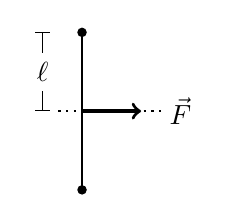
\begin{tikzpicture}
\filldraw (0,1) circle (1.5pt);
\draw (0,1) -- (0,-1);
\filldraw (0,-1) circle (1.5pt);
\draw[->,very thick] (0,0) --  (0.75,0);
\node at (1.25,0) {$\vec{F}$};
\draw[|-|] (-.5,1) to node[midway, fill = white] {$\ell$} (-.5,0);
\draw[dotted, thick] (-.3,0) -- (1,0);
\end{tikzpicture}
\end{minipage}
\begin{Answer}[ref = pucks]
	Sei $A$ das in der Aufgabenstellung gegebene System. Wir wollen nun erst einmal ein wesentlich einfacheres System $B$ betrachten. In diesem sind die beiden Pucks bereits zusammen gestoßen, und werden nur noch mit konstanter Kraft $F$ entlang der Geraden gezogen:
	\begin{figure}[h]
		\centering
		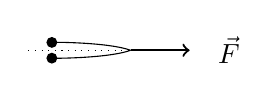
\begin{tikzpicture}
		\filldraw (0,.1) circle (1.75pt);
		\filldraw (0,-.1) circle (1.75pt);
		\draw(0.1,.1) to [out = 180, in = 160] (1,0);
		\draw(0.1,-.1) to[out=180,in = 200](1,0);
		\draw[->, thick] (1,0) --  (1.75,0);
		\node at (2.25,0) {$\vec{F}$};
		\draw[dotted, thin] (-.3,0) to (1.1,0);
		\end{tikzpicture}
	\end{figure}\\
Auf jeden der beiden Pucks wirkt hier eine Kraft $F_{(B,p)} = 1/2\cdot F$ in $x$-Richtung.\\ 
Tut sie dies während der Bewegung entlang einer Strecke der Länge $d$, so ist die Arbeit, die entlang dieses Weges an dem System $B$ geleistet wird, einfach nur $W_B = Fd$.\\
Interessant wird es, wenn wir versuchen,  auf eine ähnlich einfache Art das System $A$ aus der Aufgabenstellung zu betrachten.\\
Dazu bemerken wir zuerst, dass die Kraft $F_{(A,p),x}$ die auf einen der beiden Pucks in $x$-Richtung wirkt, auch $F_{(A,p),x} = 1/2\cdot F = F_{(B,p),x}$ ist. Das bedeutet aber, dass ein Puck im System $A$ in $x$-Richtung genau die gleiche Beschleunigung erfährt wie ein Puck im System $B$. \\
Wir können jetzt annehmen, dass man zum Zeitpunkt $t = 0$ sowohl im System $A$ als auch im System $B$ anfängt, an dem Seil zu ziehen. Dann bedeutet aber die Beobachtung, dass die Strecke, die ein Puck in $x$-Richtung nach einer Zeit $t$ zurückgelegt hat, in System $A$ und in System $B$ gleich lang ist. Gleichzeitig heißt das, dass die beiden Systeme \textit{nach} der Kollision nicht mehr unterscheidbar sind. Damit ist dann aber auch die Energie beider Systeme \textit{nach dem Stoß} im System $A$ gleich groß. \\
Sei nun $d$ die Strecke, die ein Puck im System $A$ zurück legt, bis er mit dem anderen zusammenstößt. Dann wurde an dem Seil über eine Strecke der Länge $d+\ell$ an den Pucks mit der Kraft $\vec{F}$ gezogen. Dabei müssen wir $\ell$ addieren, weil der Abstand zwischen dem Angriffspunkt der Kraft und den Pucks bei der Kollision gerade $\ell$ ist. Also ist die Arbeit, die \textit{direkt vor} der Kollision an System $A$ verrichtet wurde, genau $W_A = F(d+\ell)$.\\
Zum gleichen Zeitpunkt wurden die Pucks in System $B$ aber nur entlang einer Strecke der Länge $d$ gezogen, da sie sich ja in $B$ nur entlang der $x$-Achse bewegen. Also ist die Arbeit, die in dieser Zeit an System $B$ verrichtet wurde, gerade $W_b = Fd$.\\
Bei solchen Aufgaben kann man die Zeit, die eine Kollision benötigt, eigentlich immer vernachlässigen. Nach unserer obigen Überlegung bedeutet das aber, dass die Energie im System $A$, die \textit{nach} dem Stoß verbleibt, gerade $E'_A = W_B$ sein muss.\\
Die Differenz, $\boxed{W = W_A-E'_A = F\ell}$, ist nun gerade die Energie, die \textit{während} des Stoßes verloren gegangen seien muss.\\
Alternativ kann man auch einfach rechnen.  Betrachte dazu die Spannkraft $\vec{T}$, die auf einen Puck wirkt, in Abhängigkeit des Winkels $\theta$:
\begin{figure}[h]
	\centering
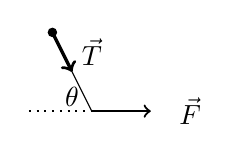
\begin{tikzpicture}
\filldraw (0,1) circle (1.5pt);
\draw (0,1) -- (0.5,0);
\draw[very thick,->] (0,1) -- (0.25,0.5); 
\node at (0.5,0.75) {$\vec{T}$};
\draw[dotted, thick] (-.3,0) -- (1,0);
\draw[->, thick] (.5,0) --  (1.25,0);
\node at (0.25,0.175) {$\theta$};
\node at (1.75,0) {$\vec{F}$};
\end{tikzpicture}
\end{figure}
Dann gilt  $T = \frac{F}{2\cos \theta}.$
Die davon in $y$-Richtung wirkende Komponente ist dementsprechend 
\begin{equation}
	T_y = -T \sin \theta = -\frac{1}{2}\cdot F\cdot \tan\theta.
\end{equation}
Darüber können wir nun integrieren, um die Arbeit $W_{y,1}$ zu errechnen, die in $y$-Richtung an dem einen Puck geleistet wurde:
\begin{align*}
	W_{y,1} = \int_{\ell}^0 \frac{-F\tan \theta}{2}~dy
	&\overset{\ast}{=} -\frac{F\ell}{2}\int_{\pi/2}^{0} \sin \theta ~d\theta\\
	&= \frac{F\ell}{2}\cdot \left. \cos \theta \right|_{\pi/2}^{0}\\
	&= \frac{F\ell}{2}, 
\end{align*}
wobei in $\ast$ die Substitution $dy = \ell \sin \theta$ genutzt wurde.\\
Da die Kraft nun aber auf beide Pucks wirkt, und wir annehmen können, dass die Pucks nur über die Schnurr miteinander wechselwirken, beträgt die gesamte in $y$-Richtung geleistete Arbeit gerade
\begin{equation*}
	\boxed{ W_y = 2W_{y,1} = F\ell }
\end{equation*}
Diese Arbeit ist aber gerade die Energie, die bei dem Stoß verloren geht.\\
Es kommt also bei beiden Ansätzen das gleiche Ergebnis raus - nett.

\end{Answer}
\begin{Exercise}[title = Lichtband, label = band, difficulty = 3, origin = {1. Runde im Auswahlwettbewerb zur IPhO 2006}]
Eine Lichtquelle in Form eines dünnen Bandes der Länge $\ell = 10~\mathrm{cm}$ liegt auf der optischen Achse einer dünnen Sammellinse der Brennweite $f = 5~\mathrm{cm}$ und dem Durchmesser $d = 1~\mathrm{cm}$. Der minimale Abstand der Lichtquelle zur Sammellinse beträgt $10~\mathrm{cm}$. Wie groß ist der minimale Durchmesser des entstehenden Lichtflecks, den die Lichtquelle auf einem senkrecht zur optischen Achse stehenden, verschiebbaren Schirm erzeugt?
\end{Exercise}
\begin{Exercise}[title = Tunnel, origin = {EstPhO 2009}, difficulty = 3, label = train]
	Ein Zug fährt mit einer Geschwindigkeit $v$ und einer Leistung $P$ durch einen langen zylindrischen Tunnel, dessen halbkreisförmige Öffnung einen Durchmesser $d$ hat.\\
	Die Anfangstemperatur im Tunnel beträgt $T_0$, der Luftdruck ist $p_0$, die molare Masse von Luft ist $M$. Während der Durchfahrt bleibt der Druck im Tunnel näherungsweise konstant. Dann ist die molare Wärmekapazität von Luft durch $C_p$ gegeben.\\
	Wie groß ist die Tunneltemperatur nach der Zugdurchfahrt?
\end{Exercise}


\end{document}